% ============================================================
%  DISCOVERY CURRICULUM — Journey 1, Module 4
%  "Sequences and Patterns"
%  Compile with: pdflatex J1_M4.tex  (run twice for references)
% ============================================================

\documentclass[12pt, a4paper]{article}

\usepackage[a4paper, top=2.8cm, bottom=2.8cm, left=3.0cm, right=2.5cm, includeheadfoot, headheight=15pt]{geometry}
\usepackage{amsmath, amsthm}
\usepackage[charter, cal=cmcal]{mathdesign}
\usepackage[scaled=0.92]{helvet}
\usepackage{xcolor}
\usepackage{tcolorbox}
\tcbuselibrary{skins, breakable, theorems}
\usepackage{enumitem}
\usepackage{graphicx}
\usepackage{tikz}
\usetikzlibrary{arrows.meta, positioning, calc}
\usepackage{pgfplots}
\pgfplotsset{compat=1.18}
\usepackage{booktabs}
\usepackage{array}
\usepackage{fancyhdr}
\usepackage{titlesec}
\usepackage{parskip}
\usepackage{microtype}
\usepackage{hyperref}
\hypersetup{colorlinks=true, linkcolor=NavyBlue, urlcolor=NavyBlue}

% ── Colours ─────────────────────────────────────────────────
\definecolor{NavyBlue}{HTML}{1E3A8A}
\definecolor{MidBlue}{HTML}{2E6DA4}
\definecolor{Gold}{HTML}{D97706}
\definecolor{LightBlue}{HTML}{EFF6FF}
\definecolor{LightGold}{HTML}{FEF3C7}
\definecolor{DarkGrey}{HTML}{334155}
\definecolor{BoxGreen}{HTML}{F0FDF4}
\definecolor{SoftRed}{HTML}{FFF1F2}
\definecolor{SidebarGrey}{HTML}{F8FAFC}

% ── Section formatting ───────────────────────────────────────
\titleformat{\section}{\Large\bfseries\color{NavyBlue}}{}{0em}{}[{\color{MidBlue}\vspace{2pt}\rule{\linewidth}{1.5pt}}]
\titleformat{\subsection}{\large\bfseries\color{MidBlue}}{}{0em}{}
\titleformat{\subsubsection}{\normalsize\bfseries\color{Gold}}{}{0em}{}

% ── Header / Footer ─────────────────────────────────────────
\pagestyle{fancy}
\fancyhf{}
\fancyhead[L]{\small\color{DarkGrey}\textit{Discovery Curriculum}}
\fancyhead[R]{\small\color{DarkGrey}\textit{Journey 1 $\cdot$ Module 4}}
\fancyfoot[C]{\small\color{MidBlue}\thepage}
\renewcommand{\headrulewidth}{0.4pt}

% ── Environments (tcolorbox Unification) ─────────────────────

% Puzzle box — opening problem
\newtcolorbox{puzzlebox}[1][]{
  enhanced, breakable,
  colback=NavyBlue!5, colframe=NavyBlue,
  boxrule=0pt, leftrule=2.5pt,
  sharp corners,
  left=12pt, right=10pt, top=10pt, bottom=10pt,
  before skip=14pt, after skip=10pt,
  #1
}

% Discovery box — moment of crystallisation
\newtcolorbox{discoverybox}[1][]{
  enhanced, breakable,
  colback=LightGold, colframe=Gold,
  boxrule=0pt, leftrule=2.5pt,
  sharp corners,
  left=12pt, right=10pt, top=10pt, bottom=10pt,
  before skip=14pt, after skip=10pt,
  #1
}

% Name box — formal definition reveal
\newtcolorbox{namebox}[1][]{
  enhanced, breakable,
  colback=LightBlue, colframe=MidBlue,
  boxrule=0.8pt,
  arc=4pt,
  left=12pt, right=10pt, top=10pt, bottom=10pt,
  before skip=14pt, after skip=10pt,
  #1
}

% Reflection box
\newtcolorbox{reflectionbox}[1][]{
  enhanced, breakable,
  colback=BoxGreen, colframe=DarkGrey!35,
  boxrule=0.8pt,
  arc=4pt,
  left=12pt, right=10pt, top=10pt, bottom=10pt,
  before skip=14pt, after skip=10pt,
  #1
}

% Thought provocation — inline philosophical aside
\newtcolorbox{thought}[1][]{
  enhanced, breakable,
  colback=SidebarGrey, colframe=Gold,
  boxrule=0pt, leftrule=1.5pt,
  sharp corners,
  left=10pt, right=10pt, top=7pt, bottom=7pt,
  before skip=10pt, after skip=10pt,
  #1
}

% Problem counter
\newcounter{problem}
\newenvironment{problem}[1][]{%
  \refstepcounter{problem}%
  \par\vspace{6pt}%
  \noindent\textbf{\color{MidBlue}Problem \theproblem}%
  \ifx&#1&\else\ \textit{(#1)}\fi\textbf{.}\enskip
}{\par\vspace{4pt}}

% Deep problem counter
\newcounter{deepproblem}
\newenvironment{deepproblem}[1][]{%
  \refstepcounter{deepproblem}%
  \par\vspace{6pt}%
  \noindent\textbf{\color{NavyBlue}$\bigstar$\ Deep Problem \thedeepproblem}%
  \ifx&#1&\else\ \textit{(#1)}\fi\textbf{.}\enskip
}{\par\vspace{4pt}}

% Exercise counter
\newcounter{exercise}
\newenvironment{exercise}[1][]{%
  \refstepcounter{exercise}%
  \par\vspace{6pt}%
  \noindent\textbf{\color{Gold}Exercise \theexercise}%
  \ifx&#1&\else\ \textit{(#1)}\fi\textbf{.}\enskip
}{\par\vspace{4pt}}

\begin{document}
% ============================================================

% ── Cover ───────────────────────────────────────────────────
\thispagestyle{empty}
\begin{center}
{\small\color{MidBlue}\textbf{DISCOVERY CURRICULUM}\quad$\cdot$\quad\textbf{JOURNEY 1: REPRESENTATION}}

\vspace{0.6cm}
{\color{NavyBlue}\rule{\linewidth}{2pt}}
\vspace{0.5cm}

{\Huge\bfseries\color{NavyBlue}Module 4}\\[0.3cm]
{\LARGE\bfseries\color{MidBlue}Sequences and Patterns}\\[0.4cm]
{\color{Gold}\rule{0.4\linewidth}{1.2pt}}\\[0.4cm]
{\large\itshape\color{DarkGrey}
A sequence is a function in disguise.\\[0.15cm]
But what happens when a sequence describes itself?}

\vspace{1cm}
\begin{tabular}{rl}
\color{DarkGrey}\textbf{Journey}           & Journey 1 --- Representation \\[4pt]
\color{DarkGrey}\textbf{Module}            & 4 of 6 \\[4pt]
\color{DarkGrey}\textbf{Prerequisites}     & Modules 1--3 (functions, composition, graphs) \\[4pt]
\color{DarkGrey}\textbf{You will discover} & Arithmetic/geometric sequences, recursion, limits of sequences, the golden ratio \\[4pt]
\color{DarkGrey}\textbf{Format}            & 8 problems $+$ 3 deep problems $\approx$ 12--14 pages \\
\end{tabular}

\vspace{1cm}
{\color{NavyBlue}\rule{\linewidth}{2pt}}
\end{center}

\vspace{0.6cm}

\noindent\textbf{Recap of Modules 1--3.}
You have built three representational languages so far: \emph{functions} (rules between sets), \emph{graphs} (patterns of connection), and the algebraic machinery connecting them. Each language strips away irrelevant detail and retains only structure.

\medskip
This module adds a fourth language: \textbf{sequences}. A sequence is simply a list of numbers ordered by position. But as you will see, sequences are functions in disguise, they encode recursive self-reference, and their long-run behaviour raises one of the most important questions in all of analysis: \emph{what happens when a process runs forever?}

\newpage

% ============================================================
\section{Part 1 \texorpdfstring{---}{--} The Puzzle}
% ============================================================

\begin{puzzlebox}
\textbf{The Opening Puzzle.}

Here are the first several terms of a sequence:
\[
1,\; 1,\; 2,\; 3,\; 5,\; 8,\; 13,\; 21,\; 34,\; 55,\; \ldots
\]

\textbf{Question 1.} What is the rule? Write it down precisely, not just in words.

\textbf{Question 2.} Compute the ratio of each term to the previous term:
$\dfrac{1}{1},\; \dfrac{2}{1},\; \dfrac{3}{2},\; \dfrac{5}{3},\; \dfrac{8}{5},\; \ldots$

What do these ratios seem to be approaching?

\textbf{Question 3.} Call the limiting ratio $\varphi$. If the ratio of consecutive terms truly approaches $\varphi$, and if the sequence satisfies its defining rule, what equation must $\varphi$ satisfy? Solve it. What number do you get?
\end{puzzlebox}

\medskip
The sequence above is ancient. It appears in Sanskrit poetry from the 6th century, in the growth patterns of nautilus shells, in the branching of trees, in the arrangement of seeds in a sunflower. The number $\varphi$ you computed has been called the golden ratio for over two millennia. Its appearance here is not decoration. It is the first hint that recursive rules --- rules that define each term using what came before --- have deeply structured long-run behaviour. Understanding that behaviour is the purpose of this module.

\begin{thought}
\textbf{Does mathematics describe nature, or does nature follow mathematics?}
The golden ratio appears in biology not because plants ``know'' mathematics, but because the Fibonacci growth rule is an efficient packing strategy that evolution discovered independently across many species. When mathematicians say a pattern ``appears in nature,'' they often mean something more cautious: the mathematical structure is a good model of the process, not that nature is consciously obeying equations. The distinction matters. One view makes mathematics a discovery about the world. The other makes it an invention we impose on the world. Mathematicians have argued about this for centuries, and there is no settled answer.
\end{thought}

% ============================================================
\section{Part 2 \texorpdfstring{---}{--} Exploration}
% ============================================================

\subsection{Step 1: The two basic types}

\begin{problem}
\label{prob:arith_geom}
Consider the following sequences. For each one:
\begin{itemize}[topsep=2pt, noitemsep]
  \item Find the pattern and write the next three terms.
  \item Write a formula for the $n$-th term $a_n$ directly in terms of $n$.
  \item Write a \emph{recursive} formula: express $a_n$ in terms of $a_{n-1}$ (or earlier terms).
\end{itemize}

\begin{enumerate}[label=(\alph*), topsep=4pt]
  \item $3,\; 7,\; 11,\; 15,\; 19,\; \ldots$
  \item $2,\; 6,\; 18,\; 54,\; 162,\; \ldots$
  \item $100,\; 50,\; 25,\; 12.5,\; \ldots$
  \item $1,\; -1,\; 1,\; -1,\; 1,\; \ldots$
  \item $1,\; 4,\; 9,\; 16,\; 25,\; \ldots$
\end{enumerate}
\end{problem}

\medskip
Sequences (a)--(d) belong to two basic families. Sequence (a) and its structure are called \emph{arithmetic}: each term is obtained by adding a fixed number. Sequences (b)--(d) are \emph{geometric}: each term is obtained by multiplying by a fixed number. Sequence (e) belongs to neither family, but has its own elegant closed form.

\begin{thought}
\textbf{Two types of growth, two types of world.}
Arithmetic sequences grow by addition: $+d$ each step. Their long-run behaviour is simple --- they grow without bound (if $d > 0$), shrink without bound (if $d < 0$), or stay constant (if $d = 0$). Geometric sequences grow by multiplication: $\times r$ each step. Their long-run behaviour is richer and more surprising. When $|r| > 1$, they explode. When $|r| < 1$, they collapse toward zero. When $r = -1$, they oscillate. When $r = 1$, they stay constant.

The difference between additive and multiplicative growth runs through all of science. Bank interest, population growth, radioactive decay, and viral spread are all geometric processes. The fact that humans systematically underestimate geometric growth --- our intuitions are wired for addition --- has real consequences in epidemiology, finance, and climate science.
\end{thought}

\begin{problem}
\label{prob:geometric_sum}
Consider the geometric sequence with first term $a$ and ratio $r \neq 1$:
\[
a,\; ar,\; ar^2,\; ar^3,\; \ldots,\; ar^{n-1}.
\]
\begin{enumerate}[label=(\alph*), topsep=2pt]
  \item Let $S_n = a + ar + ar^2 + \cdots + ar^{n-1}$. Compute $S_n - rS_n$. What do you get?
  \item Use part (a) to derive a closed formula for $S_n$.
  \item What happens to $S_n$ as $n \to \infty$ when $|r| < 1$? When $|r| > 1$?
  \item A ball is dropped from a height of 1 metre. Each time it bounces, it rises to $\tfrac{2}{3}$ of its previous height. What is the total distance the ball travels (up and down combined) before coming to rest? Does your answer surprise you?
  \item Zeno's paradox: Achilles runs at speed 1 m/s, the tortoise at $\tfrac{1}{2}$ m/s, and the tortoise starts 1 m ahead. Every time Achilles reaches where the tortoise was, the tortoise has moved a little further. Achilles must complete infinitely many steps. Does he ever catch the tortoise? Use part (c) to resolve this.
\end{enumerate}
\end{problem}

\begin{thought}
\textbf{Zeno and the infinite.}
Zeno of Elea posed his paradoxes around 450 BCE to argue that motion is an illusion. His argument is logically valid if you assume that a sum of infinitely many positive numbers must be infinite. For nearly two thousand years, no one had the mathematical tools to refute it cleanly. The resolution --- that an infinite series can converge to a finite number --- required the development of limits in the 17th century. The paradox was not silly; it was pointing at a genuine gap in the mathematics of its time. Many ``obvious'' things in mathematics turned out to require centuries of work to make rigorous. This should make you suspicious of your own mathematical intuitions.
\end{thought}

\subsection{Step 2: Sequences as functions}

\begin{problem}
\label{prob:seq_as_func}
A sequence $a_1, a_2, a_3, \ldots$ is formally a function $a : \mathbb{N} \to \mathbb{R}$, where $a(n) = a_n$.
\begin{enumerate}[label=(\alph*), topsep=2pt]
  \item Rewrite the arithmetic sequence $a_n = 3 + 4(n-1)$ as a function $a : \mathbb{N} \to \mathbb{R}$. What is the domain? What is the range?
  \item Plot the first 8 terms of the geometric sequence $a_n = 2 \cdot (0.7)^{n-1}$ on a graph with $n$ on the horizontal axis. What shape does the graph have?
  \item Plot the sequence $a_n = (-1)^n$ for $n = 1$ to $10$. How does the function picture reveal behaviour that is hard to see from the list alone?
  \item Two sequences $a_n$ and $b_n$ satisfy $a_n = 3n + 1$ and $b_n = 2n + 5$. For which values of $n$ is $a_n > b_n$? Write this as a statement about two functions.
\end{enumerate}
\end{problem}

\subsection{Step 3: Recursive rules and long-run behaviour}

\begin{problem}
\label{prob:recursion_types}
Each sequence below is defined recursively. For each one: compute the first 8 terms, plot them, and describe what happens as $n$ grows large.
\begin{enumerate}[label=(\alph*), topsep=2pt]
  \item $a_1 = 1$, \quad $a_n = a_{n-1} + 3$ \hfill (arithmetic, revisited)
  \item $a_1 = 10$, \quad $a_n = 0.9 \cdot a_{n-1}$ \hfill (geometric decay)
  \item $a_1 = 1$, \quad $a_n = 2 \cdot a_{n-1}$ \hfill (geometric explosion)
  \item $a_1 = 6$, \quad $a_n = \dfrac{1}{2}\!\left(a_{n-1} + \dfrac{12}{a_{n-1}}\right)$ \hfill (mystery rule)
  \item $a_1 = 2$, \quad $a_n = a_{n-1} \cdot \left(1 - \dfrac{a_{n-1}}{10}\right)$ \hfill (logistic rule --- harder)
\end{enumerate}

For (d): what number does the sequence approach? Can you explain why?\\
For (e): try different starting values $a_1 \in \{0.1,\, 1,\, 5,\, 9,\, 11\}$. What do you observe?
\end{problem}

\medskip
The mystery rule in (d) is Newton's method for computing $\sqrt{12}$. It works by averaging an overestimate and an underestimate, and each step roughly \emph{doubles} the number of correct decimal digits. This is called \emph{quadratic convergence}. It is one of the fastest ways to compute square roots, and variants of it underlie much of modern numerical computing.

The logistic rule in (e) is far more mysterious. Depending on the starting value, it may converge, oscillate, or behave in a way that seems completely random, despite being determined by a perfectly definite rule. This phenomenon --- \emph{deterministic chaos} --- was one of the great scientific discoveries of the 20th century, and it fundamentally changed how scientists think about predictability.

\begin{thought}
\textbf{Chaos and the limits of prediction.}
In 1961, the meteorologist Edward Lorenz discovered that tiny changes in the starting conditions of his weather model led to completely different long-term forecasts. A difference of 0.000127 in one number changed the entire simulation. This was not a computing error. It was a mathematical property of certain recursive rules: the logistic map is a simple example of the same phenomenon. The butterfly effect --- the idea that a butterfly flapping its wings in Brazil could eventually cause a tornado in Texas --- is a metaphor for this mathematical reality. The universe may be deterministic (each state determines the next exactly), and yet long-term prediction may be fundamentally impossible for certain systems. This is one of the deepest insights in 20th-century science, and it grew from studying sequences.
\end{thought}

\subsection{Step 4: The Fibonacci sequence and its ratio}

\begin{problem}
\label{prob:fibonacci}
Return to the Fibonacci sequence: $F_1 = 1,\, F_2 = 1,\, F_n = F_{n-1} + F_{n-2}$.
\begin{enumerate}[label=(\alph*), topsep=2pt]
  \item Compute $F_1$ through $F_{15}$.
  \item Compute the ratios $r_n = F_{n+1}/F_n$ for $n = 1$ to $14$. What value do they approach?
  \item If $r_n \to \varphi$, and $F_n = F_{n-1} + F_{n-2}$, divide both sides by $F_{n-1}$ and take the limit to derive the equation $\varphi$ must satisfy.
  \item Solve $\varphi^2 = \varphi + 1$. Find both solutions. What are they?
  \item The \textbf{Binet formula} claims $F_n = \dfrac{\varphi^n - \psi^n}{\sqrt{5}}$, where $\varphi$ and $\psi$ are the two solutions from (d). Verify this for $n = 1, 2, 3, 4$. Does it always give an integer? Why?
\end{enumerate}
\end{problem}

\begin{center}
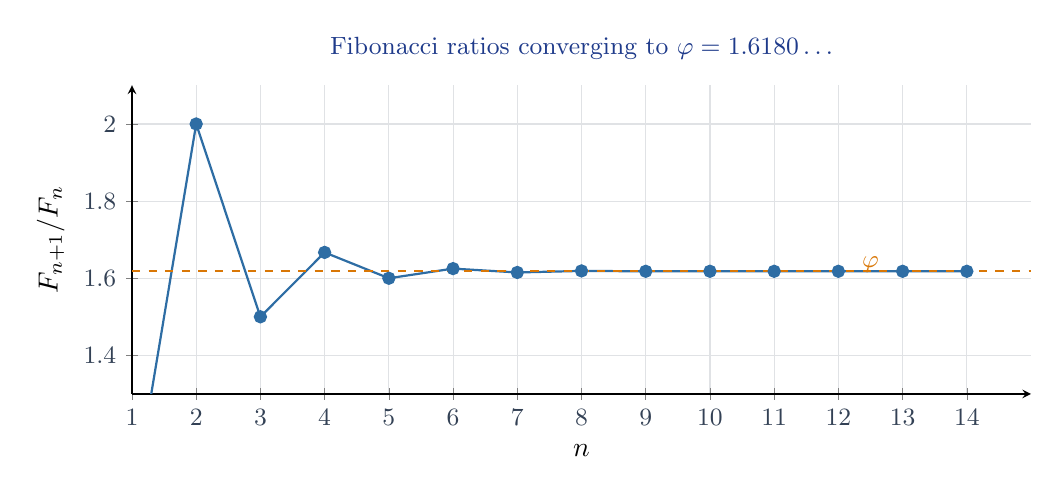
\begin{tikzpicture}
\begin{axis}[
  width=13cm, height=5.5cm,
  axis lines=left,
  xlabel={$n$},
  ylabel={$F_{n+1}/F_n$},
  xmin=1, xmax=15,
  ymin=1.3, ymax=2.1,
  xtick={1,2,...,14},
  ytick={1.4, 1.6, 1.8, 2.0},
  tick label style={font=\small, color=DarkGrey},
  grid=major, grid style={DarkGrey!15},
  title={\small\color{NavyBlue}Fibonacci ratios converging to $\varphi = 1.6180\ldots$},
]
% Fibonacci ratios: 1, 2, 1.5, 1.667, 1.6, 1.625, 1.615, 1.619, 1.618, ...
\addplot[MidBlue, thick, mark=*, mark size=2pt] coordinates {
  (1,1) (2,2) (3,1.5) (4,1.667) (5,1.6) (6,1.625)
  (7,1.615) (8,1.619) (9,1.618) (10,1.6181) (11,1.6180)
  (12,1.61804) (13,1.61803) (14,1.618034)
};
\addplot[Gold, dashed, thick, domain=1:15] {1.6180339887};
\node[color=Gold, font=\small] at (axis cs:12.5, 1.635) {$\varphi$};
\end{axis}
\end{tikzpicture}
\end{center}

\begin{problem}
\label{prob:limit_intuition}
We say a sequence $a_n$ \textbf{converges} to a limit $L$ if, for any margin of error $\varepsilon > 0$, there exists some index $N$ such that $|a_n - L| < \varepsilon$ for all $n > N$. In plain language: the terms eventually get and \emph{stay} arbitrarily close to $L$.
\begin{enumerate}[label=(\alph*), topsep=2pt]
  \item For $a_n = 1/n$: intuitively, what is the limit? Now use the formal definition: given $\varepsilon = 0.01$, find an $N$ such that $|a_n - 0| < 0.01$ for all $n > N$.
  \item For $a_n = (-1)^n$: does this sequence converge? Argue using the formal definition.
  \item For $a_n = \frac{n}{n+1}$: compute the limit. Verify it rigorously for $\varepsilon = 0.001$.
  \item For $a_n = \frac{3n^2 + 2n}{5n^2 - 1}$: what is the limit? What happens to the lower-order terms?
  \item For the Fibonacci ratios $r_n = F_{n+1}/F_n$: you have computed that they approach $\varphi$. Write an informal argument (not a full $\varepsilon$-$N$ proof) for why this must be true, based on the defining recursion.
\end{enumerate}
\end{problem}

\begin{thought}
\textbf{What is a limit, really?}
The formal definition of a limit --- the $\varepsilon$-$N$ definition you just encountered --- was not written down until the 19th century, by \textbf{Augustin-Louis Cauchy} and later made fully rigorous by \textbf{Karl Weierstrass}. For two centuries before them, Newton, Leibniz, and Euler worked with limits intuitively --- with ``infinitely small quantities'' called infinitesimals. Their results were largely correct, but their foundations were shaky. The bishop George Berkeley famously mocked the foundations of calculus, calling infinitesimals ``the ghosts of departed quantities.'' He was not entirely wrong. The $\varepsilon$-$N$ definition replaced mysticism with precision: instead of saying ``the terms get infinitely close,'' you say ``for any target accuracy, there is a point beyond which all terms hit that accuracy.'' The shift from intuition to definition is one of the great clarifications in the history of mathematics --- and it is worth sitting with the formal definition until it feels like something you could have invented yourself.
\end{thought}

\begin{problem}
\label{prob:series_intro}
A \textbf{series} is the sum of the terms of a sequence: $S = \sum_{n=1}^{\infty} a_n$. Whether this sum makes sense depends on whether the partial sums $S_N = \sum_{n=1}^{N} a_n$ converge.
\begin{enumerate}[label=(\alph*), topsep=2pt]
  \item Compute the first 6 partial sums of $\displaystyle\sum_{n=1}^{\infty} \frac{1}{2^n}$. What does this series converge to?
  \item Compute the first 6 partial sums of $\displaystyle\sum_{n=1}^{\infty} \frac{1}{n}$. Does this series converge? (Hint: compare $\frac{1}{3}+\frac{1}{4} > \frac{1}{2}$, then $\frac{1}{5}+\cdots+\frac{1}{8} > \frac{1}{2}$, and so on.)
  \item The series in (b) is called the \textbf{harmonic series}. Its divergence is surprising because $1/n \to 0$. Explain in your own words why terms going to zero is not enough to guarantee convergence.
  \item Euler showed that $\displaystyle\sum_{n=1}^{\infty} \frac{1}{n^2} = \frac{\pi^2}{6}$. Compute the first 10 partial sums numerically and verify this is plausible.
\end{enumerate}
\end{problem}

% ============================================================
\section{Part 3 \texorpdfstring{---}{--} Discovery}
% ============================================================

\begin{discoverybox}
\textbf{What have we built?}

This module has revealed four things.

\medskip
\textbf{First.} A sequence is a function $\mathbb{N} \to \mathbb{R}$. The function language from Module~1 applies immediately: domain, range, and the question of what happens as the input grows without bound.

\medskip
\textbf{Second.} Recursive definitions --- rules that define each term from previous terms --- can produce extraordinarily rich behaviour: steady convergence, oscillation, chaos, and everything in between.

\medskip
\textbf{Third.} The question ``what does this sequence approach?'' is not a vague question. It has a precise answer --- the limit --- whose formal definition captures the intuition of ``getting and staying close.''

\medskip
\textbf{Fourth.} A sum of infinitely many terms can be finite. This is not obvious, and it took two millennia to make rigorous. It is the foundation of calculus.

\medskip
\textbf{Before reading on:} The Fibonacci sequence satisfies $F_n = F_{n-1} + F_{n-2}$. This is a \emph{linear} recursive rule. The Binet formula gives $F_n$ explicitly in terms of the two solutions of $\varphi^2 = \varphi + 1$. Can you see a connection between this and what you learned about linear algebra in Module~1? What general principle might be at work?
\end{discoverybox}

% ============================================================
\section{Part 4 \texorpdfstring{---}{--} Naming the Ideas}
% ============================================================

\begin{namebox}
\textbf{Sequences and their types.}

A \textbf{sequence} is a function $a : \mathbb{N} \to \mathbb{R}$, written $(a_n)_{n \geq 1}$.

An \textbf{arithmetic sequence} has $a_n = a_1 + (n-1)d$ for a fixed \textbf{common difference} $d$.

A \textbf{geometric sequence} has $a_n = a_1 \cdot r^{n-1}$ for a fixed \textbf{common ratio} $r$.

A \textbf{recursive sequence} defines $a_n$ in terms of one or more previous terms. The Fibonacci sequence $F_n = F_{n-1} + F_{n-2}$ is the most famous example.
\end{namebox}

\begin{namebox}
\textbf{Limits of sequences.}

We write $\lim_{n \to \infty} a_n = L$ if for every $\varepsilon > 0$ there exists $N \in \mathbb{N}$ such that
\[
  n > N \;\implies\; |a_n - L| < \varepsilon.
\]
A sequence that has a limit is \textbf{convergent}; otherwise it is \textbf{divergent}.

Key facts:
\begin{itemize}[topsep=4pt, noitemsep]
  \item $\lim r^n = 0$ if $|r| < 1$; diverges if $|r| > 1$.
  \item A geometric series $\sum_{n=0}^\infty ar^n = \dfrac{a}{1-r}$ if $|r| < 1$; diverges otherwise.
  \item The harmonic series $\sum 1/n$ diverges, despite $1/n \to 0$.
  \item $\sum 1/n^2 = \pi^2/6$ (the Basel problem, solved by Euler in 1734).
\end{itemize}
\end{namebox}

\begin{namebox}
\textbf{The golden ratio.}

The \textbf{golden ratio} $\varphi = \dfrac{1+\sqrt{5}}{2} \approx 1.6180\ldots$ satisfies $\varphi^2 = \varphi + 1$.

It is the limit of the Fibonacci ratios $F_{n+1}/F_n$. The \textbf{Binet formula} gives
\[
  F_n \;=\; \frac{\varphi^n - \psi^n}{\sqrt{5}}, \qquad \text{where } \psi = \frac{1-\sqrt{5}}{2}.
\]
Note $|\psi| < 1$, so $\psi^n \to 0$, meaning $F_n$ is the nearest integer to $\varphi^n/\sqrt{5}$ for all $n \geq 1$.
\end{namebox}

% ============================================================
\section{Part 5 \texorpdfstring{---}{--} Deep Problems}
% ============================================================

\begin{deepproblem}[Solving linear recurrences]
The Fibonacci recurrence $F_n = F_{n-1} + F_{n-2}$ is a \emph{second-order linear recurrence with constant coefficients}. The method for solving it generalises beautifully.
\begin{enumerate}[label=(\alph*)]
  \item Suppose we try a solution of the form $F_n = r^n$. Substitute into the recurrence $F_n = F_{n-1} + F_{n-2}$ and show that $r$ must satisfy $r^2 = r + 1$. This is called the \textbf{characteristic equation}.
  \item The characteristic equation has two roots $\varphi$ and $\psi$. Show that the general solution is $F_n = A\varphi^n + B\psi^n$ for constants $A$ and $B$.
  \item Use the initial conditions $F_1 = 1$ and $F_2 = 1$ to find $A$ and $B$, thereby deriving the Binet formula.
  \item Solve the recurrence $a_n = 5a_{n-1} - 6a_{n-2}$ with $a_1 = 2$, $a_2 = 5$ using the same method.
  \item \textit{(Look ahead.)} The characteristic equation approach produces solutions $r^n$ --- exponential functions. Compare this to the eigenvalue problem for matrices: if $Av = \lambda v$, then $A^n v = \lambda^n v$. Can you see a connection between linear recurrences and matrix eigenvalues? This connection is made precise in Journey~3.
\end{enumerate}
\end{deepproblem}

\begin{deepproblem}[Convergence criteria]
\begin{enumerate}[label=(\alph*)]
  \item Prove rigorously that $\lim_{n \to \infty} \dfrac{1}{n} = 0$ using the $\varepsilon$-$N$ definition.
  \item Prove that if $\lim a_n = L$ and $\lim b_n = M$, then $\lim(a_n + b_n) = L + M$.
  \item A sequence $(a_n)$ is \textbf{Cauchy} if for every $\varepsilon > 0$ there exists $N$ such that $m, n > N \implies |a_m - a_n| < \varepsilon$. Explain in plain language what this means: why is being Cauchy a natural condition for convergence?
  \item Prove that every convergent sequence is Cauchy.
  \item \textit{(Harder.)} The converse --- every Cauchy sequence converges --- is called the \textbf{completeness} of $\mathbb{R}$. It is not obvious, and in fact fails for the rational numbers $\mathbb{Q}$. Can you construct a sequence of rational numbers that is Cauchy but does not converge to a rational number? What does this say about the relationship between $\mathbb{Q}$ and $\mathbb{R}$?
\end{enumerate}
\end{deepproblem}

\begin{deepproblem}[Chaos and the logistic map]
The \textbf{logistic map} is the recursion $x_{n+1} = rx_n(1 - x_n)$ for $x_n \in [0,1]$ and a parameter $r \in [0,4]$.
\begin{enumerate}[label=(\alph*)]
  \item For $r = 0.5$: starting from $x_0 = 0.4$, compute $x_1, \ldots, x_{10}$. What happens?
  \item For $r = 2.5$: same starting point. What happens now?
  \item For $r = 3.2$: compute 20 terms. Describe the long-run behaviour.
  \item For $r = 3.9$: compute 30 terms, then restart from $x_0 = 0.40001$ (a tiny change). Compare the two sequences. What do you observe?
  \item A \textbf{fixed point} of the logistic map satisfies $x^* = rx^*(1-x^*)$. Find all fixed points and determine when they are \emph{stable} (nearby sequences converge to them) versus \emph{unstable} (nearby sequences diverge from them).
  \item \textit{(Research question.)} The logistic map undergoes a \emph{period-doubling cascade}: as $r$ increases from 3, the sequence alternates between 2 values, then 4, then 8, and so on. The ratio of successive values of $r$ at which this doubling occurs converges to a constant $\delta \approx 4.669$, called the \textbf{Feigenbaum constant}. This constant appears in an enormous variety of chaotic systems, suggesting a deep universal structure. Why might a constant that appears in one simple recursion also appear in fluid turbulence, electrical circuits, and chemical reactions?
\end{enumerate}
\end{deepproblem}

% ============================================================
\section{Part 6 \texorpdfstring{---}{--} Reflection}
% ============================================================

\begin{reflectionbox}
\textbf{Your reflection task.}

\begin{enumerate}
  \item \textbf{On recursion.} The Fibonacci sequence defines each term using the two before it. In a sense, the sequence ``refers to itself.'' Can you think of other examples of self-referential definitions in mathematics, in language, or in nature? What makes self-reference powerful? What makes it dangerous?

  \item \textbf{On limits.} Before this module, you probably had an intuitive idea of what it means for a sequence to ``approach'' a value. Now you have a formal definition. Write a paragraph describing what the formal definition adds that the intuition does not. Is anything lost when intuition is replaced by formalism?

  \item \textbf{On chaos.} The logistic map is a completely deterministic rule, yet for certain values of $r$ its behaviour is unpredictable in practice. Does this change your view of what ``predictable'' means? Can a deterministic universe be unpredictable?

  \item \textbf{Looking ahead.} Module~5 studies growth and recursion in depth, including exponential functions and logarithms. Based on what you saw about geometric sequences and the logistic map, write one question you want answered about the long-run behaviour of growth processes.
\end{enumerate}
\end{reflectionbox}

\medskip
\noindent\textbf{Looking ahead.}
Module~5 takes the ideas of growth and recursion and pushes them toward their natural limits: the exponential function $e^x$, logarithms, and the surprising appearance of the number $e$ as the ``most natural'' base for growth. The recursive structure you discovered here --- and particularly the characteristic equation method for solving linear recurrences --- will reappear in Journey~2 when you study differential equations, which are the continuous analogues of recursive sequences.

\vspace{1.4cm}
\begin{center}
{\color{MidBlue}\rule{0.5\linewidth}{0.8pt}}\\[6pt]
{\small\color{DarkGrey}\textit{End of Journey 1, Module 4 --- Sequences and Patterns}}\\[4pt]
{\small\color{DarkGrey}Continue to: \textbf{Module 5 --- Growth and Recursion}}\\[6pt]
{\color{MidBlue}\rule{0.5\linewidth}{0.8pt}}
\end{center}

\end{document}